%\documentclass[a4paper, 11pt, english, twoside, openright]{article}
\documentclass[review, authoryear]{elsarticle}
 \usepackage[utf8]{inputenc}
\usepackage{lineno,amsmath}
\usepackage{graphicx}
\usepackage{url}
\usepackage{listings}
\usepackage{caption}
\usepackage{subcaption}
\usepackage{amssymb}
\usepackage{float}
\restylefloat{figure}
\usepackage{booktabs}
\usepackage{longtable}
\usepackage[hidelinks]{hyperref}
\newcommand{\sidenote}[1]{\marginpar{\footnotesize #1}} 
\newcommand{\s}{\,\mbox{s}}
\newcommand{\cm}{\,\mbox{cm}}
\newcommand{\Hz}{\,\mbox{Hz}}
\newcommand{\m}{\,\mbox{m}}
\newcommand{\mm}{\,\mbox{mm}}
\newcommand{\cmps}{\,\mbox{cm/s}}
\newcommand{\mps}{\,\mbox{m/s}}
\newcommand{\cmbps}{\,\frac{\mbox{cm}}{\mbox{s}}}
\restylefloat{table}
\usepackage{rotating}
\usepackage[margin=1in]{geometry}
\usepackage[tableposition=top]{caption}

  
\journal{Coastal Engineering}

\begin{document}
\begin{frontmatter}
\title{Experimental investigation of solitary breaking waves in the swash zone}
\author[1]{Lisa Smith}	
\author[1]{Atle Jensen}
\author[1]{Geir Pedersen}

\address[1]{ Department of Mathematics, University of Oslo, Norway}
	% Activate to display a given date or no date



\setlength{\marginparwidth}{1.1cm}

\begin{abstract}
This study presents an experimental investigation of plunging breakers on a sloping beach with an inclination of $5.1^{\circ}$. The incident waves are solitary waves with various amplitudes from non-breaking waves to plunging breakers, and the area investigated is the swash zone. PIV (Particle Image Velocimetry) is performed on images captured at four different field of views (FOV).  Shoreline position and maximum runup are measured, and are repeatable in both time and height, although  cross-sectional variations of the shoreline shape are observed at maximum runup.  For non-breaking waves the runup and fluid flow is computed by
a boundary integral techniques
combined with boundary layer model.
Then, there is excellent agreement between the experimental and the computed 
velocity profiles at the lower region of the beach, while the boundary integral technique overpredicts the maximum runup height severely. 
For breaking waves the experiments indicate that the motion becomes more irregular as we move further up the beach. In addition, there are more irregularities present  for waves with larger amplitude. Length and velocity of air bubbles entrapped by the plunger breakers are extracted from an image series captured with large a FOV. The images showed that a large air bubble remains intact for a time period during runup for the breaking waves. \\
%Surface profiles of the runup were investigated at large scale and revealed that the surface of the breaking waves were unstable for a time period during uprush.
\end{abstract}


\begin{keyword}
Breaking solitary waves, PIV, Boundary layers, Runup, Bubble entrainment.
\end{keyword}

\end{frontmatter}

\linenumbers

\section{Introduction}
In shallow water with constant depth, the nonlinear effect and dispersion will be balanced for solitary waves \citep{peregrine1983breaking}. During shoaling the wave will steepen, and at some critical  point breaking may occur. Wave breaking is one of the most important physical features in the swash zone \citep{elfrink2002hydrodynamics}. Breaking waves have a large impact on sediment transport onshore, which can result in beach erosion  and affect construction located near the shore. Although breaking waves is a well-known phenomenon from our daily life, many physical aspects regarding wave breaking are still poorly understood.

%Both computational and experimental methods have difficulties predicting tafter the wave breaking.

%Experimental work on solitary breaking wave have



 %Currently no analytical theory is able to predict the post stages of wave breaking.


 Several experimental studies of breaking waves have been performed in the recent years. A broad range of different experimental methods have been utilized to measure quantities such as surface elevation, runup, shear stress, and velocities. Techniques such as Laser Doppler Velocimetry \citep{petti01}, PIV \citep{cowen03} and application of shear sensors \citep{Barnes09}  have been utilized. The swash zone is  the region where the beach is partly wetted during runup and draw-down. Aeration and the 
small flow depth makes the swash zone a challenging region to study experimentally with the techniques mentioned above. A further development of the PIV method is Bubble image Velocimetry (BIV), which \cite{rivillas2012estimation} use to investigate velocity fields in plunging breakers. They compared the measurements with numerical simulations conducted with Reynolds Average Navier Stokes Equations Model. The   model gave fairly good agreement with the measurements in the surf zone, but the model overpredicted the velocities in the swash zone as compared to the BIV measurements. One of the latest work on solitary waves on a plane beach has been conducted by \cite{pujara2015experimental}. They investigated the flow evolution of the runup and draw-down of solitary waves in the range from non breaking to plunging breakers. A shear plate was located at different positions along the beach and measurements revealed that the maximum positive bed shear stress was obtained in the tip of the swash tongue during runup,  and was due to the evolution of a boundary layer and  bore driven turbulence. The maximum negative bed shear stress was obtained at the end of the withdrawal. The flow is accelerated during downrush by gravity and the bed shear stress increases during draw-down until a maximum was reached right before the water ran out of the measuring area.

 
%The swash zone is defined as the region where the beach is partly wetted during runup and run down.
 
%\cite{jensen2003experimental} performed an experimental investigation of wave run-up at a steep beach, where Particle Image Velocimetry (PIV) was performed when the wave front was at its steepest. They compared the measurements with a Boussinesq model. The beach slope was $10.54^\circ$ and they found that the waves with the largest amplitude was close to breaking, since a part of the wave front almost formed a plunging jet.

%\cite{petti01} did turbulence experiments of plunging and collapsing breakers. The experiments were carried out in a 48m long and 0.8m wide flume. They used  Laser Doppler Velocimetry (LDV) to measure instantaneous velocities. The velocities were measured 0.5mm above the beach bed. They concluded that turbulent energy is higher during up-rush than backwash. %They found that kolomogorov micro length scale had it maximum at the bottom of the bed. The length scale decreased towards the free surface. This is the opposite of the characteristic of plane channel flow with a free surface. 

%\citep{cowen03} used PIV with fluorescent particles to investigate the swash zone. The fluorescent particles enabled them to investigate areas where the flow was affected by air bubbles. They generated both spilling and plunging breakers with a period T=2.0s. They found that the up-rush turbulence was dominated by the bore, while the backwash was dominated by wall bounded turbulence. The experiment was conducted in a 32m long and 0.6m wide wave tank, with a beach slope with an inclination of 1:20. %The shear stress was calculated from the friction velocity, which depends on the dissipation, von karman constant and distanse to the wall.%There seems to be tendency that the up-rush friction coefficient is larger than the backwash coefficients. 

%A large and medium scale measurement of bed shear stress in bore driven swash was conducted by \cite{Barnes09}. They used a shear plate, based on a shear cell developed by \cite{grass1995shear}. The surface of the shear plate was smooth and with dimensions 10cm x 20cm. The medium scale experiment was done in a 20m long and 0.45m wide flume. The slope was 1:10 and two different grades of roughness were employed at the beach. The large scale experiment was done in a 20m long and 0.85m wide flume. Experiments were done with different roughness and the beach had a slope of 1:12.   The results revealed that the bed shear stress had its maximum value at the bore arrival and then decreased with time. The backwash maximum was about 2-4 times less than the up-rush maximum, which is in accordance to \cite{cowen03}. 

% \cite{kikkert11} did measurements on a bore driven swash. The experiments were carried out in a 20m long flume with a width of 0.45m. They used PIV to measure velocities and Laser-Induced Fluorescence (LIF) to measure the water depth. The beach slope was 1:10 and the experiments were repeated on beaches with different roughness. This study concludes that the up-rush friction factors are smaller than friction factors for backwash. This contradicts the findings from the work done by \cite{cowen03} and \cite{Barnes09}. \cite{rivillas2012estimation} used Bubble image Velocimetry (BIV) to investigate velocity fields in the swash and surf zone for plunging breakers. A numerical model based on Reynolds Average Navier Stokes (RANS) equation was used to compare the measurements. \cite{rivillas2012estimation} found that the BIV measurements were in agreement with the RANS model. 

Until now, PIV measurements with high temporal resolution close to the beach 
have not been reported for plunging breakers waves in the swash zone. 
This paper 
presents PIV measurements for solitary waves, of different amplitudes, that 
ranges from non-breaking to plunging cases. The paper starts with a description of the experimental set-up
 and the computational Boundary Integral Model used in this study (chapter \ref{experimnetal-set-up}). Further on,  measured and computed results will be presented; the surface elevation of the incident waves in chapter \ref{surf_elev}, surface development and maximum runup in chapter \ref{max_run}, velocity profiles from the swash zone in chapter \ref{vel_pro}, and air bubble investigation in chapter \ref{bub_inv}. Finally, a discussion of the findings will be presented in chapter \ref{con_rem}.

\section{Experimental set-up and formulation}
\label{experimnetal-set-up}

\subsection{The wave tank}
\label{wavetank}

The experiments were conducted in  a $25\m$ long and $0.51\m$ wide wave tank 
located at the Hydrodynamics Laboratory at the University of Oslo.
Incident waves were generated in an equilibrium depth of $H=20.5\cm$ by
a piston type wave maker using the method described in 
\cite{jensen2003experimental}. 
A PETG (Polyethylene Terephthalate Glycol-modified) beach with an inclination of $5.1^{\circ}$ was placed in the wave tank with its toe $529.81\cm$ from the start position of the wave paddle. Two coordinate systems are introduced, one parallel to the still water level $(x',z')$, and one parallel to the beach $(x,z)$ (see Figure \ref{fig:beach_tegning}).  The origin of both is at the equilibrium shoreline.

Nominally, the amplitude to depth ratios should equal $(\alpha=0.10,0.12,0.20,0.30,0.40,0.50)$.  
However, imperfection in the generation and frictional effects along
the wave tank reduced the heights slightly such that the amplitude in front of the
beach, $A$, became slightly less than $\alpha H$.  
An acoustic wave gauge (ultra Banner U-Gage S18U, sample frequency of $200Hz$) measured the wave height at the toe of the beach and the Boundary Integral Method (BIM) was used to correct for  the influence of the reflected wave.
The resulting amplitudes are given in table \ref{tab:max_shore}.


\begin{figure}[]
\centering
\includegraphics[width=\textwidth]{./Figures/setup3.png}
%http://commons.wikimedia.org/wiki/File:Breaking_wave_types.gif
\caption{\textit{ Sketch of  the experimental set-up.}}
\label{fig:beach_tegning}
\end{figure}

\subsection{Instrumentation, measurements}
\label{ins_measure}
To obtain velocity fields in the swash zone, high speed video was recorded at four different field of views (FOV), located upward along the beach (Table \ref{tab:loc}).  The water in the tank was seeded with polymid particles with diameters of approximately $50$ $\mu$m. A Quantronix Darwin Duo pulsed laser generated a light sheet parallel to the centreline of the wave tank, and a Photron SA5 high speed camera (1024 x 1024) synchronized with the laser, captured images of the illuminated particles. A Carl Zeiss Makro- Planer 2/50 zf ($50\mm$) lens was used. Images were collected at 3000 frames per seconds ($fps$).
 \begin{table}[]
 \centering
\caption{\textit{Location of the different FOVs  in $\cm$. The dimensions of the FOVs are approximately $4\cm$ x $4\cm$.}}
\begin{tabular}{|c|c|c|c|c|c|c|}
\hline
\textbf{FOV:}      & I                   & II                 & III     & IV \\ \hline
\textbf{Location, x:}& {[}8.49 - 13.04{]} & {[}36.35 - 40.26{]} & {[}77.55 - 81.53{]} & {[}117.76 - 121.80{]} 
 \\ \hline
\textbf{Location, z:}&  {[}-0.05 - 3.78{]} & {[}-0.16 - 3.54{]} & {[}-0.04 - 3.79{]} & {[}-0.85 - 3.09{]} 
\\ \hline
\end{tabular}
\label{tab:loc}
\end{table}
The image processing were performed in DigiFlow \citep{digiflow}. PIV was performed using interrogation windows of 32 x 8 pixels with a 75\% overlap. Oblong interrogation windows are beneficial in boundary layer flow and have been employed previously in \cite{liu2007boundary} and \cite{pedersen2013runup}. A temporal averaging of 10 images was applied to reduce noise from the data. The number of images used in the average was carefully selected, such that the mean results were not affected by the averaging.\sidenote{Must be more specific} 

To investigate air bubbles encapsulated by the plunging breakers, the camera was moved further away from the wave tank, resulting in much larger FOV than the FOVs installed to obtain velocity fields. This FOV will be referred to as FOV A and covers $0\cm< x <60\cm$. The frame rate was reduced to  500 $fps$  
and a continuous dedolight 400D was used as illumination, replacing the laser. A white background sheet was attached to the side wall of the wave tank and the water was dyed dark blue to increase the contrast of the images.

The maximum runup was measured by capturing images of the shoreline at its maximum position. A high speed Photron APX  camera was mounted on rails above the beach in the wave tank with same inclination as the beach. A high pulsed white light was used as illumination. The camera captured 125 frames per second, and the maximum shoreline profiles were tracked manually for each wave. All the experiments were repeated at least three times. The scatter $\delta_i$ for some measured quantity $x_i$, is then calculated in the following manner,

\begin{equation}
\delta_i=\frac{x_i-\overline{x}}{\overline{x}},
\end{equation}

where $\overline{x}$ is the mean over the repetitions.


To find a measure of the irregularities present in the PIV measurements, the standard deviations of the velocities are calculated for the strongest plunging breaker. Deviations are extracted at times where the mean flow, $u$, in an area near the beach has a velocity close to either
$40$, $0$ or $-40$, all measured in $\cmps$.
\begin{equation}
\sigma=\sqrt{\frac{1}{N-1}\sum_{i=1}^{N}(x_i-\overline{x})^2}, 
\end{equation}
where $N$ is the number of repetitions.
The average deviations in the $z$-direction are calculated from the area ($0\cm < z \le 0.6\cm$)
\begin{equation}
\overline{\sigma}=\sqrt{\frac{1}{M}\sum_{j=1}^{M}\sigma_j^2},
\label{av_g}
\end{equation}
where $M$ corresponds to number of  grid points in the given $z$-range.

\subsection{The potential flow and boundary layer models}
The evolution of the waves during shoaling, as well as the runup for the smallest amplitude, were 
computed by a BIM (Boundary Integral Model) for  inviscid flow \citep{pedersen2013runup}. This model may accurately describe the runup of fully nonliear non-breaking waves and the evolution of plunging breakers.
However, the model breaks down when a plunger re-attaches with fluid or impacts the beach. Moreover, the
model  becomes singular when the contact angle at the shoreline exeeds $90^\circ$  and the results  become unreliable for contact angles slightly smaller than this.  

The potential flow model also provides the outer flow and the pressure gradient
which are used as input to a FDM viscous boundary layer model. However, the coupling between the
models is only one way as there is no feed-back from the boundary layer to the potential
flow model. 
More details on both models are given in \cite{pedersen2013runup}. 

For $\alpha=0.1$ a refinement of the spatial grid resolution of from a typical value of $0.14H$ to half this size  gave a change of 0.9\% in the runup height. 
Since the BIM model is of fourth (space) and third (time) order this point to an error for the finer resolution which is much smaller than 1\%. The same resolutions were applied to the breaking waves.  For all the waves the temporal 
increment for the finest grid was $0.0073\s$, which is twice as large as the temporal averaging interval  used in the PIV processing. The viscous boundary layer model generated 600 grid points along the beach, with a spatial increment of $0.0042H$. The time resolution was kept the same as for the BIM.


\section{Results}
\label{result}

Visual inspection of the experiments revealed that the cases with normalized amplitude $\alpha=0.10$ and $\alpha=0.12$ did not break until the draw-down, while all the other cases developed into plunging breakers at, or before, the equilibrium shoreline. The plunger breakers encapsulated large amounts of air, which resulted in air bubbles in the swash tongue of the breaking waves (Figure \ref{fig:boble_bevis}).

\begin{figure}[]
\centering
\scalebox{1}[-1]{\includegraphics[angle=180,width=0.7\textwidth]{./Figures/BUBBLE/new_jan_bilde_bub.eps}}
%http://commons.wikimedia.org/wiki/File:Breaking_wave_types.gif
\caption{\textit{Image of the swash tongue for $\alpha=0.50$. The camera is tilted with the same inclination as the beach, and the swash tongue propagates from left to right.}}
\label{fig:boble_bevis}
\end{figure}

\subsection{Surface elevation of the incident waves}
\label{surf_elev}
The amplitude of the smallest wave is determined by
a simple correction scheme. First the maximum of the series from the 
acoustic gauge $A_m$ is used as solitary wave amplitude in the BIM model.
For the lowest wave this value is $A_m/H=0.0998$.
When BIM data are extracted at the gauge position we obtain 
a slightly too large surface elevation $A_b=0.1008$, due to the reflection from 
the beach. We then adjust the amplitude 
according to $A=A_m (1- \frac{ (A_b-A_m)}{A_m})$. 
The result is $A/H=0.09865$ and the comparison with BIM results, obtained with this amplitude for the incident wave, is shown in Figure \ref{fig:surf_ele1}.
The surface elevation measurements are in close agreement with computed surface elevation from the BIM simulations. 
When the surface elevation of the incident waves are very steep, the ultra sonic signal will not get reflected back and registered by the sensor. 
This leads to dropouts in the measurements, which have been filled in by linear interpolation.  Cubic polynomial regression is used to remove noise from the signal.  The corrected and measured amplitudes for all the  waves are given in Table \ref{tab:max_shore}.



\begin{figure}
\centering
\includegraphics[width=0.4\textwidth]{./Figures/surf_ele10_2016.eps}
%http://commons.wikimedia.org/wiki/File:Breaking_wave_types.gif
\caption{\textit{Measured and computed surface elevation for $\alpha=0.10$.}}
\label{fig:surf_ele1}
\end{figure}


\subsection{Surface development and maximum runup}
\label{max_run}

BIM simulations of the near-shore evolution model is shown in Figure \ref{fig:BIM}.
For reasons explained previously we only compute the runup for the 
smallest wave, $\alpha=0.10$.  For the other cases shown the numerical
model describes the evolution of the plunger, but nothing beyond its impact onshore.  
\begin{figure}[]
\centering 
\includegraphics[width=0.5\textwidth]{./Figures/BIM/case10_BIM_runup.eps}
\includegraphics[width=0.5\textwidth]{./Figures/BIM/case20_BIM_runup.eps}
\includegraphics[width=0.5\textwidth]{./Figures/BIM/case30_BIM_runup.eps}
\includegraphics[width=0.5\textwidth]{./Figures/BIM/case40_BIM_runup.eps}
\includegraphics[width=0.5\textwidth]{./Figures/BIM/case50_BIM_runup.eps}
%http://commons.wikimedia.org/wiki/File:Breaking_wave_types.gif
\caption{\textit{BIM simulation of the waves the upper to lower figures correspond to $\alpha=(0.10, 0.20, 0.30, 0.40, 0.50)$, respectively. In the top panel the curve marked 3 corresponds to the time of maximum runup.}}
\label{fig:BIM}
\end{figure}

For $\alpha=0.1$ the computed time, inundation length and height for  
maximum runup  
were $t=8.93\s$, $r=112.78\cm$ (measured along the beach), and $R/A=4.95$ 
respectively. 
Comparing this the the measurements in Table \ref{tab:max_shore} we observe that the theoretical runup height is  30\%  too large and and occurs $0.07\s$ later.   \cite{pedersen2013runup} reported differences that were similar, but smaller, deviations
between experiments and potential flow soloutions which they suggested were caused by the lack of viscous effects and surface tension in the model. The dicreapancies of  \cite{pedersen2013runup} were presumably smaller than those herein because the 
beach was steeper in the reference ($10.54 ^\circ$) which led to thicker flow depths and shorter inundations. 
In fact, in Figure \ref{fig:max_runup} we observe transverse variations in the experiments and the average
runup height is more than 5\% smaller than the maximum one, which implies that real difference between theoretical and computed
runup is larger than indicated by the maximum values. Table \ref{tab:max_shore} shows that the maximum runup is fairly repeatable for all waves including the breaking ones. % An image of shoreline at maximum runup for case 10 is shown in \ref{fig:overflate_10_bilde}.  

\begin{table}[]
\caption{\textit{Amplitudes and runup. $A$ is incident wave amplitude, $A_m$ is the maximum measured surface elevation at the toe of the beach, $r$ is the inundation length , $R$ is the vertical maximum runup, $t$ is the time corresponding to max runup and $e$ is the estimated deviation in the measurement.}}
\centering
\begin{tabular}{cccccccc}
\hline
      $\alpha$&  $A/H$&   $A_m/H$&  $r [\cm]$ &$R/A$ & $e_r [\%]$ & $t$ & $e_t [\%]$ \\ \hline
\textit{$0.10$} &\textit{$0.0986$}  &\textit{$0.0998$}  & 87.25    &    3.82  & 1.68             & 8.86 s        & 0.15              \\
\textit{$0.12$}  &\textit{$0.1184$}  &\textit{$0.1194$}  & 105. 67   &    3.85   & 0.27             & 8.67 s        & 0.15               \\
\textit{$0.20$}  &\textit{$0.1977$}  &\textit{$0.1984$} & 147.37    &    3.22  & 0.93            & 8.53 s        & 0.31                \\
\textit{$0.30$}  &\textit{$0.2959$}  &\textit{$0.2967$}  & 191.67     &   2.80  & 1.08           & 8.03 s        & 0.78              \\
\textit{$0.40$}  &\textit{$0.3930$}  &\textit{$0.3936$}  & 227.42      &   2.50 & 0.11            & 7.82 s        & 0              \\
\textit{$0.50$}  &\textit{$0.4863$}  &\textit{$0.4869$}  & 267.46       &    2.37 & 2.27            & 7.30 s        & 1.64              
\end{tabular}
\label{tab:max_shore}
\end{table}

The shoreline at maximum runup are shown in Figure \ref{fig:max_runup}. It is fairly repeatable for the amplitude close to $0.1$ times the 
depth, but has a wedge-like shape. 
 This is presumably due to a cross-wise deformation  of the beach 
which has been measured using a straightedge and a feeling gauge. 
The typical maximum suppression in each transect of the beach was $3\mm$. If we assume that the depressions were unsystematic and that the later
stages of runup are governed by gravity alone (see, for instance, \cite{jensen2003experimental}) this should correspond to a variation
 of $3\cm$ on a 1 in 10 slope beach. However, even though the
flow depth is small during runup, the momentum transport due to
 the pressure is still noticeable (inferred from the simulations, results not shown). More importantly, there is a systematic suppression at the center-line of the beach and the beach width is $51\cm$, which is comparable to the inundation length for the smallest amplitude. 
Hence, another relevant estimate of the runup variation is the suppression times the contact angle (angle of fluid wedge during runup) in $radians$. In the simulations this angle approaches $0.5^\circ$ at maximum runup, which yields a variation in $x$ of $30\cm$. This is modified by 
surface tension that affects the contact angle and 
shape of fluid body near the shoreline. Unfortunately, we cannot
quantify this effect from the experiments.  
From Figure 
\ref{fig:max_runup} it is clear that transverse variation is larger than the first estimate, but smaller than the latter one. The runup varies much more for the three repetitions of the breaking wave $\alpha=0.50$,
resulting in irregularly shaped shorelines  (Figure \ref{fig:max_runup}).
\begin{figure}[]
        \centering
        \makebox[\linewidth][c]{%
        ~ %add desired spacing between images, e. g. ~, \quad, \qquad, \hfill etc.
          %(or a blank line to force the subfigure onto a new line)
        \begin{subfigure}[H]{0.4\textwidth}
                \includegraphics[width=0.95\textwidth]{Figures/runup10.eps}
        \end{subfigure}
         %add desired spacing between images, e. g. ~, \quad, \qquad, \hfill etc.
          %(or a blank line to force the subfigure onto a new line)
        \begin{subfigure}[H]{0.4\textwidth}
                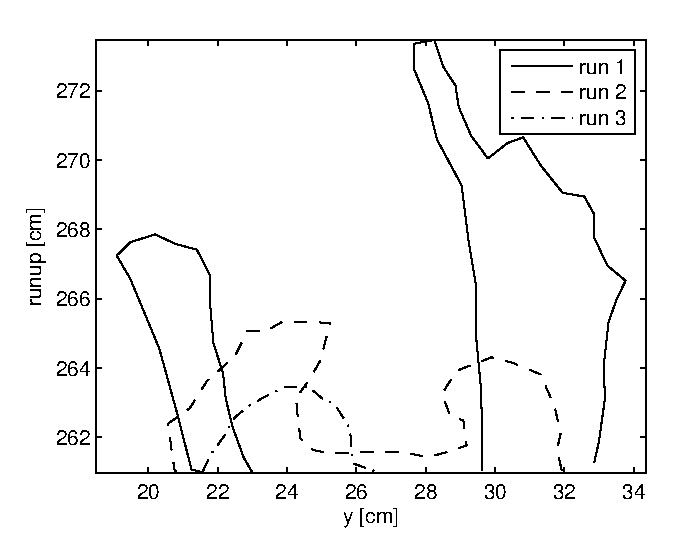
\includegraphics[width=0.95\textwidth]{Figures/runup50.eps}
        \end{subfigure}
}
        \caption{\textit{Cross-sectional variation of the shoreline shapes at max runup. Left: $\alpha=0.10$, Right: $\alpha=0.50$.}}
        \label{fig:max_runup}
\end{figure}

An estimate of the arrival time of the wave for FOV II, III and IV, were calculated from intensity changes in the image captured at the different FOV.  Each image in each time series was compared to the initial image taken before the wave paddle starts. The image where the sum of the light intensity differs more than a given threshold (1000)\sidenote{1000 what ?} from the initial image, correspond to the time when the wave enters that FOV. The measured shoreline positions as a function time are presented in Figure \ref{fig:arr_tim}. The maximum error obtained for three different runs was 0.18\%. This indicate that the shoreline motion was repeatable for each of the FOV.
\begin{figure}
        \centering
        ~ %add desired spacing between images, e. g. ~, \quad, \qquad, \hfill etc.
          %(or a blank line to force the subfigure onto a new line)
                \includegraphics[scale=0.6]{./Figures/shoreline2016.eps}
                \caption{\textit{Shoreline position as a function of time for all cases. The first measurements correspond to the swash tongue arrival time for FOV II, III, IV. The last measuring point for all cases correspond to measurement of maximum runup.}}
              \label{fig:arr_tim}
      \end{figure}


\subsection{Velocity profiles from the swash zone}
\label{vel_pro}

Velocity profiles are extracted from the PIV data that are obtained from the four different FOVs, 
approximately from $10\cm$ to $120\cm$ from the equilibrium shoreline. 
In figure \ref{fig:BIM3_tim}) we observe that computed (BIM) and measured (PIV) velocity profiles agree for $\alpha=0.10$ in FOV I and II.  The maximum deviation between measured and computed outer flow occured at the beginning of PIV timeseries and was 4.7\% and 6.8\% for FOV I and II (not shown), respectively. The deviations decreased for both FOVs as time increased.  This complies with corresponding results in \cite{pedersen2013runup} where the
delay of the experimental wave was linked to capillary effects, while
an accumulative reduction of velocity, and hence runup height, was
related to the viscous boundary layers further up the beach.  Hence, the BIM 
computation over-predicts the maximum runup as given in the previous section.

\begin{figure}
        \centering
        ~ %add desired spacing between images, e. g. ~, \quad, \qquad, \hfill etc.
          %(or a blank line to force the subfigure onto a new line)
                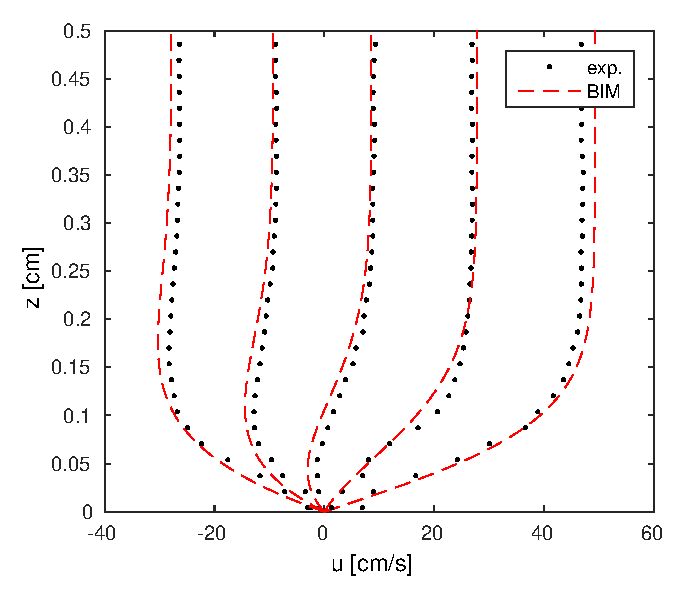
\includegraphics[width=0.3\textwidth]{./Figures/BIM/case10_BIM_PIV_FOV3.eps}
                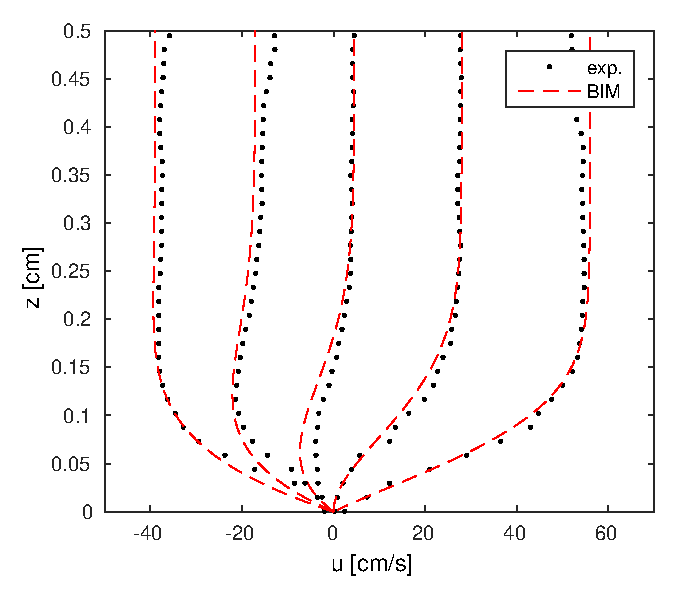
\includegraphics[width=0.3\textwidth]{./Figures/BIM/case10_BIM_PIV_FOV4.eps}
                \caption{\textit{ Velocity profiles for $\alpha=0.10$.\\ Left: FOV I $x=8.7\cm$ $t=[7.48, 7.82, 8.15, 8.48, 8.81]\s$.\\
                 \quad Right: FOV II $x=40.1\cm$ $t=[7.76, 8.10, 8.76, 9.10]\s$.}}
              \label{fig:BIM3_tim}
      \end{figure}
      
\begin{figure}
        \centering
        ~ %add desired spacing between images, e. g. ~, \quad, \qquad, \hfill etc.
          %(or a blank line to force the subfigure onto a new line)
               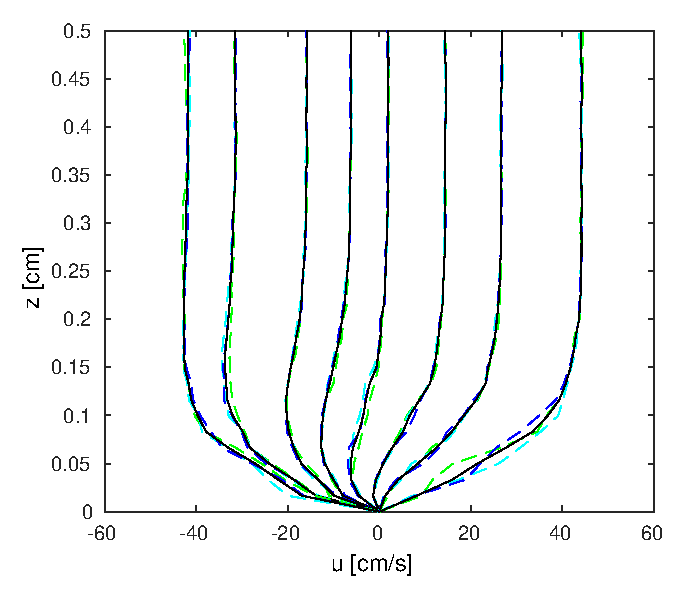
\includegraphics[width=0.3\textwidth]{./Figures/BIM/case50_BIM_PIV_FOV3.eps}
                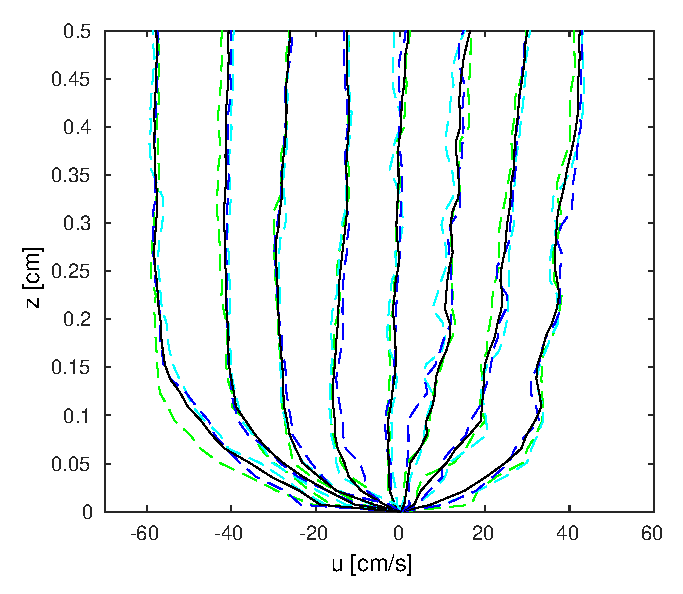
\includegraphics[width=0.3\textwidth]{./Figures/BIM/case50_BIM_PIV_FOV4.eps}
                \\
                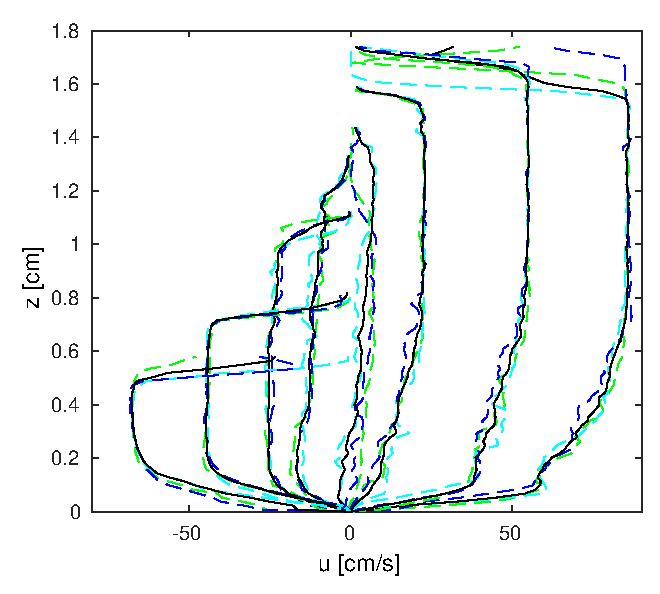
\includegraphics[width=0.3\textwidth]{./Figures/BIM/case50_BIM_PIV_FOV5.eps}
                 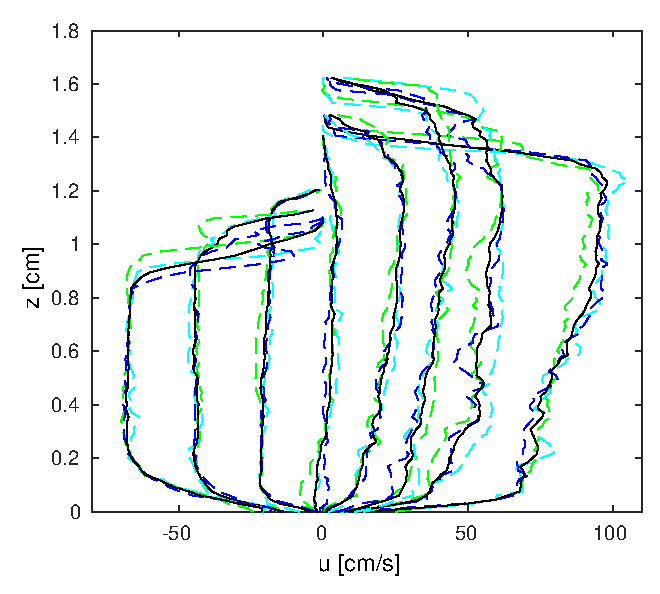
\includegraphics[width=0.3\textwidth]{./Figures/BIM/case50_BIM_PIV_FOV6.eps}
                \caption{\textit{Velocity profiles for $\alpha=0.50$. Colors: blue, cyan and green correspond to run 1,2 and 3. \\Upper Left: FOV I $x=8.7cm$ $t=[6.12, 6.34, 6.50, 6.69, 6.84, 7.00, 7.27, 7.45]\s.$\\
                 \quad Upper Right: FOV II $x=40.1cm$ $t=[6.43, 6.57, 6.74, 6.92, 7.14, 7.36, 7.56, 7.80]\s.$\\
                  \quad Lower Left: FOV III $x=81.4cm$ $t=[6.34, 6.60, 6.94, 7.12, 7.34, 7.50, 7.80, 8.16]\s.$\\
                   \quad Lower Right: FOV IV $x=121.2cm$ $t=[6.50, 6.78, 6.94, 7.10, 7.32, 7.60, 7.91, 8.20]\s.$}}
              \label{fig:plot50}
      \end{figure}



 
%When a viscous fluid flows near a flat plate, a boundary layer can be obtain. Boundary layers are caused by viscous effect of the fluid and are also due to no-slip condition at the plate. Since there is a smooth transition from this trancient velocity area to the area of constant velocity, there is no defined line between boundary layer and the outer flow, but often is the boundary layer described as the area from the plate to the streamline where  $u =0.99U$.

 %Velocity profiles from the swash zone,  during flow reversal will be presented from FOV I,II and III. In addition, will the results be compared with a BIM boundary layer solution for the smallest waves, $A/H=0.0989$. 


%Underneath the solitary waves generated in this investigation, a boundary layer were obtained close to the beach (Figure \ref{fig:PIV_FOV4}). This can be interpreted that viscous effects are of great importance in analysis of swash tongues. Especially since the boundary layer occupying a large portion of the swash tongue thickness. The event of a swash tongue moving with a velocity U upward a beach can be compared to the problem of accelerating an infinite long plate from rest to a constant velocity U with a viscous fluid on top (Stokes first problem). Dimensional analysis gives us the relationship $\delta \approx \sqrt{\nu t}$.
%By introducing dimensional analysis to this problem an approximation to the boundary layer thickness can be found. If a flat plate suddenly accelerate to a velocity U, it will take some time for the motion to diffuse into the fluid on top. As a result the length of the area affected by the plate change in velocity (boundary layer thickness $\delta$) must be dependent on the time since the incident.The viscosity of the fluid will also affect how large the boundary layer will become.



%Velocity profiles for non-breaking solitary waves are studied experimentally by \cite{pedersen2013runup}.Their measurements revealed that the velocity profiles obtained close to the still water shoreline, had a viscous boundary layer close to the beach, and a uniform velocity U outside the boundary layer (the outer flow). 
The PIV analysis of the breaking waves was difficult due to air bubbles in the flow, and due to challenges with particle seeding within the thin swash zone.  The case $\alpha=0.50$ has the longest runup of all the breaking waves, and that makes it the one for which 
 most data can be extracted from all the FOVs. Velocity profiles for $\alpha=0.50$ are shown in Figure \ref{fig:plot50}. The velocity profiles are extracted at times after all the air bubbles have passed each of the FOV. It is clear that the velocities at FOV I resembles the velocities obtained for $\alpha=0.10$. The boundary layer is well defined and the deviation between the different runs is really small. For FOV II-IV the deviations tends to increase as we move further up the beach. However the largest irregularities are in
 runup phase, while they are decreases in the retreating flow. Hence, the withdrawal fase has a more regular boundary layer and a well defined outer flow for all the FOVs. The scatter parameter $\overline{\sigma}$, defined in (\ref{av_g}) is presented in Table \ref{tab:irr}. The findings substantiate the interpretation made of the data shown in Figure \ref{fig:plot50}.


\begin{table}[]
\caption{\textit{The irregularity measure, $\overline{\sigma}$, for $\alpha=0.50$.}}
\centering
\begin{tabular}{ccccccc}
\hline
FOV& $  u\sim40\cmbps$  &$ u\sim 0\cmbps$ & $u\sim -40\cmbps$   \\ \hline
\textit{I}  & 1.04   &    0.33  & 0.67                       \\
\textit{II}  & 1.13   &    0.65   & 1.12                    \\
\textit{III} &  2.26   &    1.11 &  1.06                            \\
\textit{IV}  & 3.88    &   2.00  & 0.97                 \\
\end{tabular}
\label{tab:irr}
\end{table}



The velocities near flow reversal for all the different wave amplitudes will be discussed in the following. FOV II is located approximately $40\cm$ from the origin, and velocity 
profiles obtained from this FOV are shown in Figure \ref{fig:PIV_FOV4}.
For $\alpha=0.20$ the particle density was too sparse close to the surface, which led to spurious vacillations in the velocity profiles near  $z\approx1$. Some distance below the surface a region of uniform flow is apparent for all cases. 
Boundary layers are apparent for all the cases and they all
display a flow reversal prior to that of the outer flow.
However, the evolution of the boundary layers for 
$\alpha\le 0.2$ and those for $\alpha\ge 0.3$ differ.
The boundary layers for the higher amplitudes appear more irregular
with a thicker and less pronounced region of reversed flow in the 
boundary layers. 
While the boundary layer for the lower amplitudes, including that of $\alpha=0.20$, appears laminar the higher waves have boundary layers that 
presumably are in a transition to turbulence.   

\begin{figure}[]
\centering
\makebox[\linewidth][c]{%
\begin{subfigure}[b]{.3\textwidth}
\centering
\includegraphics[width=.95\textwidth]{./Figures/BIM/profil10_feb.eps}
\caption{\textit{$\alpha=0.10$}}
\end{subfigure}%
\begin{subfigure}[b]{.3\textwidth}
\centering
\includegraphics[width=.95\textwidth]{./Figures/BIM/profil12_feb.eps}
\caption{\textit{$\alpha=0.12$}} 
\end{subfigure}%
\begin{subfigure}[b]{.3\textwidth}
\centering
\includegraphics[width=.95\textwidth]{./Figures/BIM/profil20_feb.eps}
\caption{\textit{$\alpha=0.20$}}
\end{subfigure}%
}
\makebox[\linewidth][c]{%
\begin{subfigure}[b]{.3\textwidth}
\centering
\includegraphics[width=.95\textwidth]{./Figures/FOV_4/case30_sept2015.eps}
\caption{\textit{$\alpha=0.30$}}
\end{subfigure}%
\begin{subfigure}[b]{.3\textwidth}
\centering
\includegraphics[width=.95\textwidth]{./Figures/FOV_4/case40_sept2015.eps}
\caption{\textit{$\alpha=0.40$}}
\end{subfigure}%
\begin{subfigure}[b]{.3\textwidth}
\centering
\includegraphics[width=.95\textwidth]{./Figures/FOV_4/case50_sept2015.eps}
\caption{\textit{$\alpha=0.50$}}
\end{subfigure}%
}
\caption{ \textit{FOV II, mean velocity profiles before and after the outer flow reverses ($\triangle$,$\bigcirc$,$\square$). Colors: blue, cyan, green and red correspond to run 1,2,3 and BIM respectively.  $x=40.1\cm$. } }
\label{fig:PIV_FOV4}
\end{figure}
 FOV III is located about $80\cm$ from origo along the beach. For $\alpha=0.10$ and $\alpha=0.12$, the swash tongues were too thin, and particles within the tongue were impossible to detect. Consequently, only $\alpha=0.20-0.50$ will be presented for this FOV. None of the cases had an outer flow with constant velocity at times close to outer flow reversal \sidenote{What is the flow depth ?}(see Figure \ref{fig:PIV_FOV5}). This indicates that the motion was more irregular for this FOV than for FOV II.
 \begin{figure}[]
\centering
\makebox[\linewidth][c]{%
\begin{subfigure}[b]{.3\textwidth}
\centering
\includegraphics[width=.95\textwidth]{./Figures/FOV_5/PIV_FOV5_case20.eps}
\caption{$\alpha=0.20$}
\end{subfigure}%
\begin{subfigure}[b]{.3\textwidth}
\centering
\includegraphics[width=.95\textwidth]{./Figures/FOV_5/PIV_FOV5_case30.eps}
\caption{$\alpha=0.30$}
\end{subfigure}%
}
\makebox[\linewidth][c]{%
\begin{subfigure}[b]{.3\textwidth}
\centering
\includegraphics[width=.95\textwidth]{./Figures/FOV_5/PIV_FOV5_case40.eps}
\caption{$\alpha=0.40$}
\end{subfigure}%
\begin{subfigure}[b]{.3\textwidth}
\centering
\includegraphics[width=.95\textwidth]{./Figures/FOV_5/PIV_FOV5_case50.eps}
\caption{$\alpha=0.50$}
\end{subfigure}%
}
\caption{ \textit{FOV III, mean velocity profiles before and after the outer flow reverses ($\triangle$,$\square$). Colors: blue, cyan and green correspond to run 1,2 and 3. 
$x=81.4\cm$}. }
\label{fig:PIV_FOV5}
\end{figure}

 FOV IV is located about $120\cm$ from where the still water reaches the beach. At this FOV, only $\alpha=0.30-0.50$ will be presented due to the thin swash tongue for the other waves. Velocity profiles are given in Figure \ref{fig:PIV_FOV6}. The velocity was less repeatable at this location than for the other FOVs. The velocity profiles were more irregular, especially for $\alpha=0.50$, where the average velocity profile obtained before flow reversal is reminiscent of the parbolic velocity profiles from fully developed turbulent channel flow, as described in \cite{white2006viscous}. %For laminar channel flow the velocity profiles has parabolic shape, and as the reynold number increases to fully developed turbulent channel flow, the velocity profiles has a larger area in middle of the channel where the velocity is constant. The velocity decays closer to the walls for turbulent regimes than for the laminar flow regimes. The mean velocity profile obtained for $A/H=0.4874$ has a shape that resembles the time average velocity profile for turbulent channel flow in addition to a frequent fluctuating velocity around this mean.

%The shape of the velocity profiles seems to differ more from the shape observed for the non-breaking solitary waves in \citep{pedersen2013runup} as we move further up the beach. In addition, it seems like stronger breakers differs more from the non-breaking shape, than the small breakers. Overall, the velocities before and after flow reversal, seemed to become more irregular as the waves washes up the beach.  
\begin{figure}[]
\centering
\makebox[\linewidth][c]{%
\begin{subfigure}[b]{.3\textwidth}
\centering
\includegraphics[width=.95\textwidth]{./Figures/FOV_6/PIV_FOV6_case30.eps}
\caption{\textit{$\alpha=0.30$}}
\end{subfigure}%
\begin{subfigure}[b]{.3\textwidth}
\centering
\includegraphics[width=.95\textwidth]{./Figures/FOV_6/PIV_FOV6_case40.eps}
\caption{\textit{$\alpha=0.40$}}
\end{subfigure}%
\begin{subfigure}[b]{.3\textwidth}
\centering
\includegraphics[width=.95\textwidth]{./Figures/FOV_6/PIV_FOV6_case50.eps}
\caption{\textit{$\alpha=0.50$}}
\end{subfigure}%
}
\caption{\textit{FOV IV, mean velocity profiles before and after the outer flow reverses ($\triangle$,$\square$). Colors: blue, cyan and green correspond to run 1,2 and 3. 
$x=121.2\cm$}. }
\label{fig:PIV_FOV6}
\end{figure}
\begin{figure}[]
        \centering
        ~ %add desired spacing between images, e. g. ~, \quad, \qquad, \hfill etc.
          %(or a blank line to force the subfigure onto a new line)
                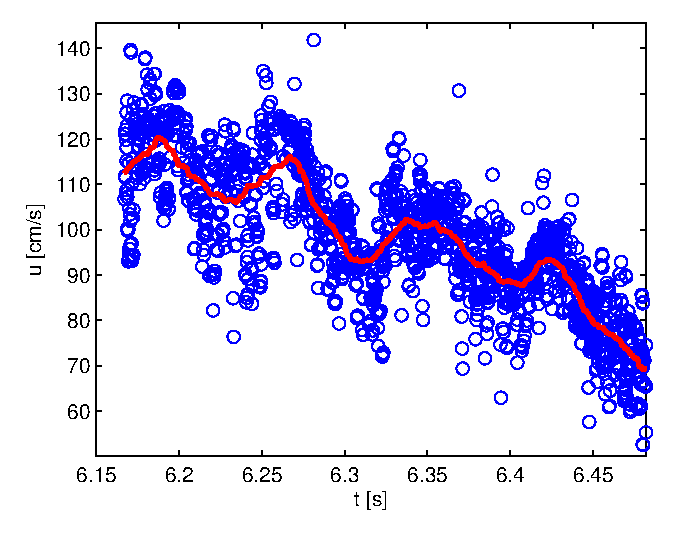
\includegraphics[scale=0.6]{./Figures/tid_case50_run2.eps}
                \caption{\textit{FOV IV Collection of velocities of particles within a distance of $0.05\cm$ from the point $(x,z)=(120,0.3)\cm$. The data is collected from  $\alpha=0.50$, run 2. Blue circles: Raw data points. Red line: 2 order interpolation with 40 evaluation points}.}
                \label{fig:wave_in_time}
        \end{figure}      

Inspection of videos of the front of the swash tongue from FOV IV (furthest up the beach) indicates that a systematic swirling effect were present in the front of the swash tongue for $\alpha=0.50$. To investigate this phenomenon, Particle Tracking Velocimetry (PTV) has been utilized on images captured close to arrival of the swash tongue ($5.33\s$). There were sparse particle seeding in the front of the tongue, and the first time where enough particles were present for an ensemble PTV analysis, was at $t=6.16\s$. This is still long before the large bubble arrives at this FOV. For each image pair after this, the velocity for all the particles within a distance of $0.05\cm$ from a given evaluation point $(x,y)=(120\cm,0.3\cm)$ are assessed. Figure \ref{fig:wave_in_time} shows how the velocities vary as a function of time. Superimposed a steady deceleration of the fluid there is an 
oscillation.
Flow in decelerating boundary layers are prone to instabilities.
However, the oscillations do not increase in magnitude and are present
from the beginning. 
   This indicates that the wave breaking induces irregularities, possibly in the form of vortices, that prevails during the subsequent motion. 


 
 \subsection{Bubble investigation}
 \label{bub_inv}
 For the plunging breakers ($\alpha=0.20-0.50$) one large air bubble is encapsulated. As the waves propagated upward the beach, this bubble disintegrated into smaller and smaller bubbles. Before maximum runup, all the 
bubbles have escaped the surface. The images captured with the large FOV A provides some information about this air bubble formation (see Figure \ref{fig:bubble_30} and \ref{fig:bubble_50}). To enhance the shape of the bubbles the gradient magnitude image is represented. The shape of the main bubble is oval with a thin tongue in the front, for $\alpha=0.30$. The shape of the main air bubble appears less repeatable for $\alpha=0.50$. In particular, in run 2 the large air bubble cannot
 be identified in the image at all. The length of the main bubble for three different runs is given in Table \ref{tab:b_case30}. It is clear from the images and Table \ref{tab:b_case30}, that the three different runs are more similar for $\alpha=0.30$ than for $\alpha=0.50$. This supports the assertion that larger plungers are more irregular.
 
The air bubble velocity in the direction along the beach is given in Table \ref{vel_bubb}. The largest velocities were obtained in the front of the bubbles for most of the runs, and may explain the shape of the thin tongue in the front of the air bubble observed for $\alpha=0.30$. The bubbles velocities can be compared to the velocities of the developing shoreline (Figure \ref{fig:arr_tim}). The average shoreline velocity from  FOV II to FOV III was found to be $1.87\mps$ for $\alpha=30$ and $2.75\mps$ for $\alpha=50$, and the average is taken within a time interval close to the times of the bubble investigation. The average shoreline motion was smaller than the average bubble velocity for $\alpha=30$, which interpret that the bubbles will not be lagged relative to the swash tongue for this wave, and the bubbles may not affect the later stages of the runup as much as first assumed. However for $\alpha=0.50$ the average bubble velocity is smaller than the shoreline velocity which makes  the area where air bubbles are present will be extended. This may be one of the reasons for the large irregularities measured with the PIV system in the beginning of the swash tongue (see Figure \ref{fig:plot50}).
\begin{figure}[]
\centering
\includegraphics[width=0.7\textwidth]{./Figures/BUBBLE/bubble_30_run1.eps}
\includegraphics[width=0.7\textwidth]{./Figures/BUBBLE/bubble_30_run2.eps}
\includegraphics[width=0.7\textwidth]{./Figures/BUBBLE/bubble_30_run3.eps}
%http://commons.wikimedia.org/wiki/File:Breaking_wave_types.gif
\caption{\textit{Gradient magnitude images of the swash tongue for $\alpha=0.30$, run 1, 2 and 3. $t=6.06\s$. The red line shows the length of the main air bubble}.}
\label{fig:bubble_30}
\end{figure}


\begin{figure}[]
\centering
\includegraphics[width=0.6\textwidth]{./Figures/BUBBLE/bubble_50_run1.eps}
\includegraphics[width=0.6\textwidth]{./Figures/BUBBLE/bubble_50_run2.eps}
\includegraphics[width=0.6\textwidth]{./Figures/BUBBLE/bubble_50_run3.eps}
%http://commons.wikimedia.org/wiki/File:Breaking_wave_types.gif
\caption{\textit{Gradient magnitude images of the swash tongue for $\alpha=0.50$, run 1, 2 and 3. $t=5.54\s$. The red line shows the length of the main air bubble}.}
\label{fig:bubble_50}
\end{figure} 


\begin{table}[]
\centering
\caption{\textit{ Size of the main bubble measured at $t=6.06\s$ for $\alpha=0.30$, and $t=5.54\s$ for $\alpha=0.50$}.}
\label{my-label}
\begin{tabular}{|c|c|c|c|}
\hline
\textbf{Main bubble size }              & \textbf{Run 1 {[}$\cm${]}} & \textbf{Run 2 {[}$\cm${]}} & \textbf{Run 3 {[}$\cm${]}} \\ \hline
$\alpha=0.30$:  & 8.00     & 8.94     & 7.90     \\ \hline
$\alpha=0.50$: & 9.24     &      & 8.17     \\ \hline
\end{tabular}
\label{tab:b_case30}
\end{table}
 
%\begin{table}[]
%\centering
%\caption{Size of the main bubble measured at t=5.54s for case 50}
%\label{my-label}
%\begin{tabular}{|c|c|c|c|}
%\hline
%\textbf{Run}              & \textbf{1} & \textbf{2} & \textbf{3} \\ \hline
%Main bubble size {[}cm{]} & 9.2426     & 7.5314     & 8.2136     \\ \hline
%\end{tabular}
%\label{tab:b_case50}
%\end{table}
 
\begin{table}[]
\centering
\caption{\textit{ Velocities along the beach for the main air bubble. $t=6.06\s$ for $\alpha=0.30$, and $t=5.54\s$ for $\alpha=0.50$}.}
\label{vel_bubb}
\begin{tabular}{llll}
\hline
{\bf $\alpha=0.30$}                    & Run 1 & Run 2 & Run 3 \\ \hline
Front velocity {[}$\mps${]}  & 2.05  & 2.20  & 2.48  \\
Tail velocity {[}$\mps${]}  & 2.10  & 2.05  & 2.23  \\ \hline
{\bf $\alpha=0.50$}                    &       &       &       \\ \hline
Front velocity {[}m/s{]}  & 3.26  &   & 2.01  \\
Tail velocity {[}m/s{]}   & 1.58  &   & 2.23 
\end{tabular}
\end{table} 
 
 
%\begin{table}[h]
%\center
%\begin{tabular}{|l|l|l|l|}
%\hline
%{\bf $A/H=0.2958$}            & {\bf Run 1} & {\bf Run 2} & {\bf Run 3} \\ \hline
%Front velocity {[}m/s{]} & 2.05        & 2.20        & 2.48        \\ \hline
%Tail velocity {[}m/s{]}  & 2.10        & 2.05        & 2.23        \\ \hline
%{\bf Case 50}            & {\bf Run 1} & {\bf Run 2} & {\bf Run 3} \\ \hline
%Front velocity {[}m/s{]} & 3.26       &2.58        & 2.01        \\ \hline
%Tail velocity {[}m/s{]}  & 1.58         & 2.40        & 2.23        \\ \hline
%\end{tabular}
%\caption{My caption}
%\label{my-label}
%\end{table} 
 
%\begin{table}[h]
%\centering
%\begin{tabular}{|l|l|l|l|}
%\hline
%{\bf Case 50}            & {\bf Run 1} & {\bf Run 2} & {\bf Run 3} \\ \hline
%Front velocity {[}m/s{]} & 3.26       &2.58        & 2.01        \\ \hline
%Tail velocity {[}m/s{]}  & 1.58         & 2.40        & 2.23        \\ \hline
%\end{tabular}
%\caption{My caption}
%\label{my-label}
%\end{table} 
 
\section{Discussion}
\label{con_rem}

For runup of non-breaking solitary waves on a $5.1^\circ$ slope we 
observe laminar boundary layers. The presumption of laminarity is
 supported by the good agreement found with boundary layers computed 
by combining a potential flow model with a standard boundary layer model on the beach. However, in accordance with \cite{pedersen2013runup} the
potential flow model overpredicts the
maximum runup height by  30\%.  
The discrepancies between computations and measurements, which probably are due to viscosity and capillary effects, are in reality larger since tiny deformation of the beach increases the maximum runup height in the experiments.

The measurement of the breaking waves showed that the fluid motion becomes more irregular and less repeatable as we move further up the beach. In addition, the motion was more irregular for the waves with the stronger plunger than for those with smaller amplitude. The maximum runup was fairly repeatable, but marked an irregular
transverse  variations were observed for the breaking waves. The bubble investigation indicated
 that the air bubble shapes  were repeatable  for the waves with amplitude $\alpha=0.30$ but not for the waves with amplitude $\alpha=0.50$. Overall, irregular motion increases with larger breaking waves and as the waves propagate upwards the beach.  

\section*{Acknowledgment}

This work was funded by the Research Council of Norway through the research project DOMT - Developments in Optical Measurement Technologies (project number 231491).

\section*{References}
\bibliographystyle{elsarticle-num}
 \bibliography{bibliography}

\end{document}

